\documentclass[conference]{IEEEtran}
\IEEEoverridecommandlockouts
% The preceding line is only needed to identify funding in the first footnote. If that is unneeded, please comment it out.
%----------------------------------------------------------
\usepackage{cite}
\usepackage[pdftex]{graphicx}
\usepackage{siunitx}
% declare the path(s) where your graphic files are
\graphicspath{images/}
\DeclareGraphicsExtensions{.pdf,.jpeg,.png,.jpg}
\usepackage{amsmath,amssymb,amsfonts}
\usepackage{algorithmic}
\usepackage{graphicx}
\usepackage{textcomp}
\usepackage{array}
%\usepackage[caption=false,font=normalsize,labelfont=sf,textfon =sf]{subfig}
\usepackage{dblfloatfix}
\usepackage{url}
\usepackage{lipsum}
\usepackage{listings}
\usepackage{xcolor}
\def\BibTeX{{\rm B\kern-.05em{\sc i\kern-.025em b}\kern-.08em
    T\kern-.1667em\lower.7ex\hbox{E}\kern-.125emX}}
%----------------------------------------------------------
    \lstset{
        escapeinside={/*@}{@*/},
        language=Python,	
        basicstyle=\fontsize{8.5}{12}\selectfont,
        numbers=left,
        numbersep=2pt,    
        xleftmargin=2pt,
        frame=tb,
        columns=fullflexible,
        showstringspaces=false,
        tabsize=4,
        keepspaces=true,
        showtabs=false,
        showspaces=false,
        morekeywords={inline,public,class,private,protected,struct},
        captionpos=b,
        lineskip=-0.4em,
        aboveskip=10pt,
        extendedchars=true,
        breaklines=true,
        prebreak = \raisebox{0ex}[0ex][0ex]{\ensuremath{\hookleftarrow}},
        keywordstyle=\color[rgb]{0,0,1},
        commentstyle=\color[rgb]{0.133,0.545,0.133},
        stringstyle=\color[rgb]{0.627,0.126,0.941},
    }
%----------------------------------------------------------

\begin{document}

\title{Trocando mensagens\\
{\footnotesize \textsuperscript{*} Sistemas Embarcados: Prof. Marco Reis - marco.reis@ba.docente.senai.br}
}

% \author{\IEEEauthorblockN{Marco Reis, 41650-010\IEEEauthorrefmark{1}}
% \IEEEauthorblockA{\IEEEauthorrefmark{1}Robotics & Autonomous Systems Center,
% Senai Cimatec, Salvador, Brazil}% <-this % stops an unwanted space

\author{
    \IEEEauthorblockN\centerline{}{Ludmila Nascimento Dos Anjos}
    \IEEEauthorblockA{\textit{Graduanda em Engenharia Elétrica} \\
        \textit{SENAI CIMATEC}\\
        Salvador, Bahia \\
        ludmila.n.anjos@gmail.com}
    \and
}
\maketitle

\begin{abstract}
    This document is a model and instructions for \LaTeX.
    This and the IEEEtran.cls file define the components of your paper [title, text, heads, etc.]. *CRITICAL: Do Not Use Symbols, Special Characters, Footnotes,
    or Math in Paper Title or Abstract.
\end{abstract}

\begin{IEEEkeywords}
    Arduino, Comunicação Serial, Sistema Embarcado, LCD, Sensor ultrassônico
\end{IEEEkeywords}

\section{Introdução}

\subsection{Contexto}

\subsection{Justificativa}

\subsection{Porquê}

\subsection{Importância}

\subsection{Objetivos}
O objetivo do projeto trocando mensagens é a construção de um sistema utilizando dois arduinos,
onde um deles medirá a distância entre um objeto e um sensor ultrassônico, sinalizando a região onde o objeto se encontra através de led's,
e enviará a informação de distância como o tipo string via comunicação serial, para ser disponibilizada em um display LCD conectado ao segundo arduino.

\section{Referencial teórico}
Nesta seção serão apresentados os dispositivos, e a forma de comunicação, utilizadas para o desenvolvimento do projeto.

\subsection{Arduino}
A placa de circuitos arduino \ref{fig:arduino} é uma plataforma de prototipagem eletrônica de hardware livre, cuja linguagem de programação tem fortes semelhanças com
as linguagens C/C++. Segundo Cavalcante, 2011 \cite{cavalcante2011} resumidamente, ela a consiste em uma placa com entradas e saídas para um microcontrolador AVR, um 
ambiente de desenvolvimento (Arduino IDE) e o bootloader que já vem gravado no microcontrolador. 

Dentro de sua estrutura de entradas e saídas ela possui duas portas de comunicação serial que utilizam o protocolo UART (\textit{Universal asynchronous receiver/transmitter}), 
Tx e Rx. Onde o TX é responsável pela emissão de dados e o RX pela recepção deles. No presente projeto há a comunicação entre dois arduinos utilizando dessa conexão.

\begin{figure}[htbp]
    \centerline{
        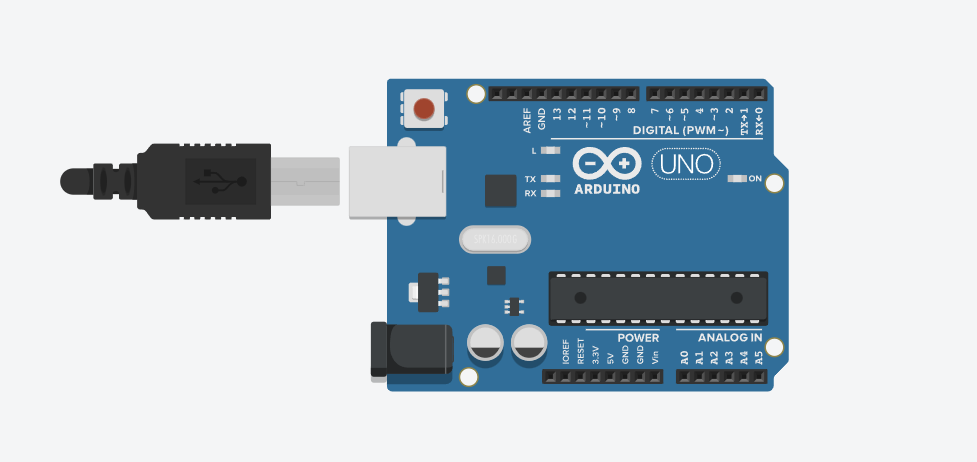
\includegraphics[width=6cm]{images/arduino.png}
    }
    \caption{Arduino Uno R3.}
    \label{fig:arduino}
\end{figure}

\subsection{Medição de distância através do Sensor ultrassônico}

O sensor ultrassônico \ref{fig:ultrassonico} é um dispositivo utilizado para medir distâncias através do valor de tempo registrado entre a emissão e recepção de uma 
onda ultrassônica. O tempo é obtido utilizando-se a função \textit{pulseIn( int pinoReceptordoSinal, int intensidadedoPulso)}, que envia um pulso e retorna o valor de 
tempo. Segundo \cite{nakatani2014}, o sensor transmite 8 ciclos de pulsos ultrassônicos a 40 kHz e espera pelo sinal refletido, medindo uma distância de 2 cm a 400 cm,
com uma precisão de até 0,3 cm, sendo que essa distância pode ser calculada através da \ref{eq:1}

\begin{figure}[htbp]
    \centerline{
        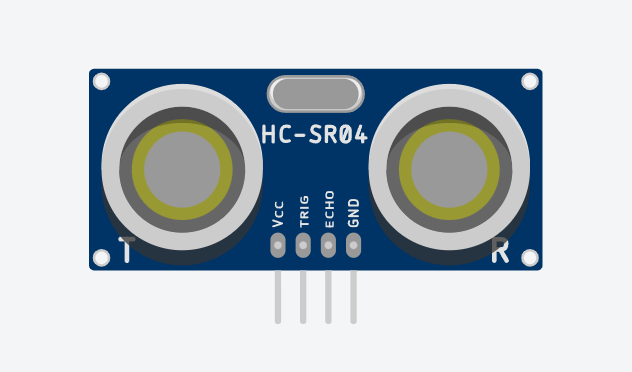
\includegraphics[width=4cm]{images/sensor-ultrassonico.png}
    }
    \caption{Sensor Ultrassônico.}
    \label{fig:ultrassonico}
\end{figure}


\begin{equation}
    distancia = tempo * velocidade do som / 2 \label{eq:1}
\end{equation}

\subsection{Display LCD(Liquid crystal display)}
Um display de cristal líquido, é um dispositivo de painel fino utilizado para exibir informações através da comunicação de dados de bits por via eletrônica como 
imagens, textos e vídeos. O LCD 12X2 \ref{fig:display} tem um fundo azul e escrita branca, possuindo 16 colunas e 2 linhas para escrita. Segundo Barbacena 1996 
\cite{barbacena1996display}, há nele 16 pinos para conexão, sendo eles pinos de alimentação do módulo, ajuste de contraste, seleção, dados e alimentação da luz de fundo.

\begin{figure}[htbp]
    \centerline{
        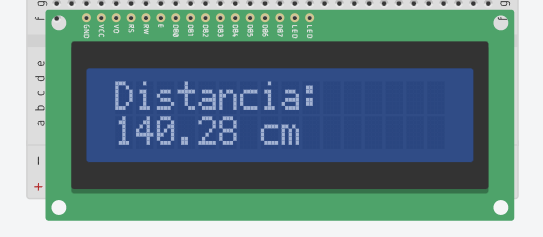
\includegraphics[width=5cm]{images/display.png}
    }
    \caption{Display LCD 16x2.}
    \label{fig:display}
\end{figure}

\subsection{Potenciômetro}
O potenciômetro \ref{fig:potenciometro} pode ser definido como uma resistência variável. Desse modo ele tem a capacidade de variar a corrente de um circuito e o brilho
de um led. Segundo Patsko 2006  \cite{patsko2006}, ele é composto por uma faixa de material resistivo (geralmente grafite) ligada entre seus dois terminais externos, 
nela há um cursor que a depender da alteração de sua posição é alterada a resistência entre o terminal e os dois terminais externos do dispositivo. 

\begin{figure}[htbp]
    \centerline{
        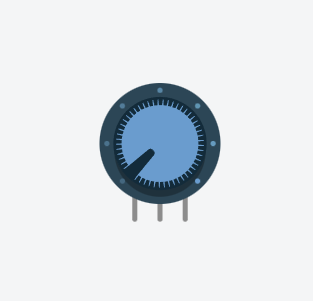
\includegraphics[width=3cm]{images/potenciometro.png}
    }
    \caption{Potenciômetro.}
    \label{fig:potenciometro}
\end{figure}

\section{Metodologia}

\subsection{Materiais}
Os materiais de hardware utilizados para a elaboração do projeto foram:
\begin{itemize}
    \item 2 arduinos UNO;
    \item 2 protoboards;
    \item 1 potenciômetro;
    \item 1 display de LCD;
    \item 1 sensor ultrassônico HC-SR04;
    \item 32 jumpers;
    \item 1 LED azul;
    \item 1 LED vermelho;
    \item 1 LED amarelo;
    \item 3 resistores de 220 \si{\ohm};
    \item 1 resistor de 1 K \si{\ohm};
\end{itemize}
Os softwares utlizados foram:
\begin{itemize}
    \item Tinkercad;
    \item Arduino IDE;
\end{itemize}

\subsection{Métodos}

Realizou-se as conexões dos dispositivos ao arduino no simulador tinkercad conforme o mostrado na figura 1.
Então, foi efetuada a programação de ambos os arduinos. O arduino 1 foi programado para captar dados do sensor ultrassônico, tratá-los
e conforme a distância em centímetros identificada acender um led azul, vermelho e amarelo para representar a região ao qual se encontra o objeto, sendo que a região mais próxima é a região 3, representada pelo led azul.
Além disso, ele também envia a informação sobre a distância de um objeto como string via comunicação serial para o arduino 2, que por sua vez utiliza de um display lcd, com regulação de brilho via potenciômetro, para mostrar a informação.

Em seguida, após a confecção do modelo virtual foi montado o circuito físico(Figura 2) com os mesmos materiais de hardware e com a mesma programação inserida nos dois arduinos através do software arduino IDE e uma conexão com um notebook.


\begin{figure}[htbp]
    \centerline{
        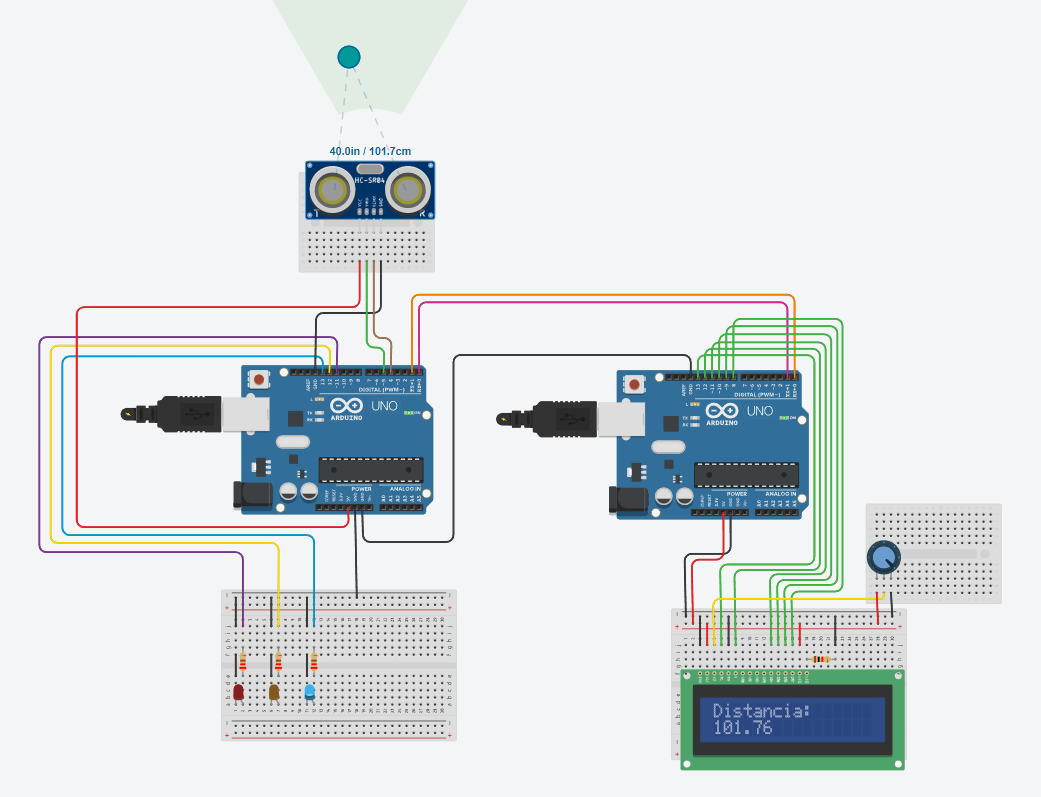
\includegraphics[width=4cm]{images/esquema-arduino.png}
    }
    \caption{Esquematico do sistema.}
    \label{fig}
\end{figure}

\begin{figure}[htbp]
    \centerline{
        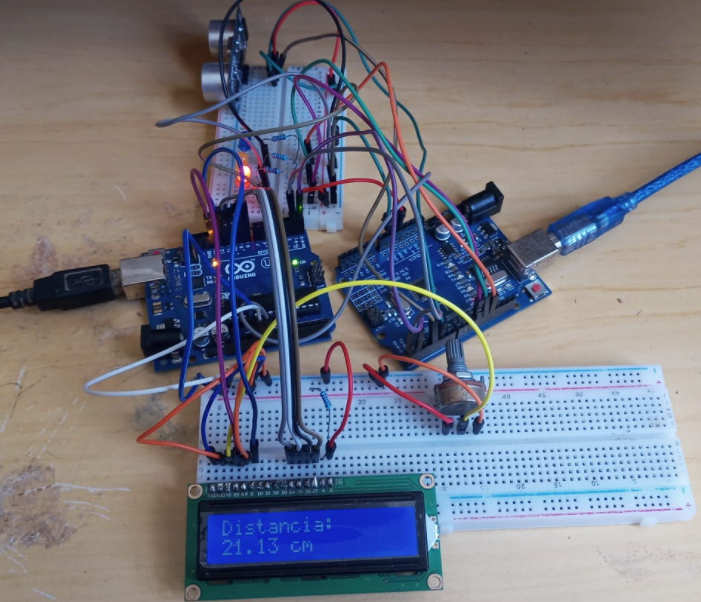
\includegraphics[width=4cm]{images/esquema-arduino-fisico.png}
    }
    \caption{Protótipo físico do sistema.}
    \label{fig}
\end{figure}

\section{Resultados e Análises}

\subsection{Montagem do circuito}

Na montagem do esquemático do circuito virtual no simulador Tinkercad não ocorreu nenhuma dificuldade relacionada à conexão entre componentes.
Diferentemente da montagem do circuito físico, pois, devido ao mau contato entre as ligações os dados passados para o display estiveram corrompidos. Para solucionar este problema jumpers precisaram ser substituídos
e o display precisou ser soldado a um suporte para conectá-lo à protoboard.

\subsection{Efeito do delay}
Notou-se que o valor utilizado na função delay afetou drasticamente a comunicação serial entre os dois arduinos, a forma encontrada para contornar isso foi utilizar a função delayMicroseconds. Pois, esta afeta menos ao tempo de comunicação do sistema.

\subsection{Finalização da comunicação}
Foi necessário o envio de uma sinalização de quebra de linha para o sistema do arduino receptor do pacote de informação para o mesmo identificar quando ocorreu o término da chegada do pacote.

\subsection{Leitura do sensor ultrassônico HC-SR04}

O sistema físico do arduino master ao receber dados referente ao tempo para a captação da reflexão de uma onda de som ultrassônico realizou o cálculo da distância entre o objeto e o sensor.
Foi perceptível a pequena oscilação entre os valores obtidos de distância, isso ocorreu pois o sensor não possuí filtros eletrônicos específicos e estava sujeito a interferência causada por outras ondas sonoras no ambiente.

Devido a essa oscilação, a forma utilizada para diminuir a alteração no valor de distância mostrado no display LCD foi mostrar nele a média de 10 valores lidos.

\section{Conclusão}
Conclui-se que os sensor ultrassônico HC-SR04 possui um erro associado a sua leitura devido a fatores internos e externos.
Além disso, que o contato adequado entre os componentes proporiona uma comunicação da informação corretamente. Ainda conclui-se que, o pacote de informação precisa ter algo para sinalizar que foi completamente enviado.
Dessa forma, o projeto se apresentou como uma excelente forma de compreender o funcionamento de dispositivos eletrônicos e sua comunicação.

\bibliographystyle{IEEEtran}
\bibliography{Bibliography}

\end{document}
